\chapter{Quantum computing and cryptography
I}\label{Quantum-computing-and-cryptogr}

\begin{quote}
\emph{``I think I can safely say that nobody understands quantum
mechanics.''} , Richard Feynman, 1965
\end{quote}

\begin{quote}
\emph{``The only difference between a probabilistic classical world and
the equations of the quantum world is that somehow or other it appears
as if the probabilities would have to go negative''}, Richard Feynman,
1982
\end{quote}

For much of the history of mankind, people believed that the ultimate
``theory of everything'' would be of the ``billiard ball'' type. That
is, at the end of the day, everything is composed of some elementary
particles and adjacent particles interact with one another according to
some well specified laws. The types of particles and laws might differ,
but not the general shape of the theory. Note that this in particular
means that a system of \(N\) particles can be simulated by a computer
with \(poly(N)\) memory and time.

Alas, in the beginning of the 20th century, several experimental results
were calling into question the ``billiard ball'' theory of the world.
One such experiment is the famous ``double slit'' experiment. Suppose we
shoot an electron at a wall that has a single slit at position \(i\) and
put somewhere behind this slit a detector. If we let \(p_i\) be the
probability that the electron goes through the slit and let \(q_i\) be
the probability that conditioned on this event, the electron hits this
detector, then the fraction of times the electron hits our detector
should be (and indeed is) \(\alpha = p_iq_i\). Similarly, if we close
this slit and open a second slit at position \(j\) then the new fraction
of times the electron hits our detector will be \(\beta=p_jq_j\). Now if
we open both slits then it seems that the fraction should be
\(\alpha+\beta\) and in particular, ``obviously'' the probability that
the electron hits our detector should only \emph{increase} if we open a
second slit. However, this is not what actually happens when we run this
experiment. It can be that the detector is hit a \emph{smaller} number
of times when two slits are open than when only a single one hits. It's
almost as if the electron checks whether two slits are open, and if they
are, it changes the path it takes. If we try to ``catch the electron in
the act'' and place a detector right next to each slit so we can count
which electron went through which slit then something even more bizarre
happened. The mere fact that we \emph{measured} the electron path
changes the actual path it takes, and now this ``destructive
interference'' pattern is gone and the detector will be hit
\(\alpha+\beta\) fraction of the time.


\begin{marginfigure}
\centering
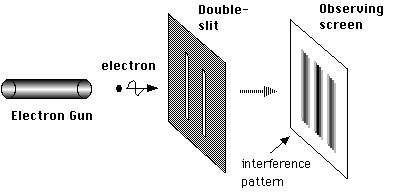
\includegraphics[width=\linewidth, height=1.5in, keepaspectratio]{../figure/double-slit-setup.PNG}
\caption{The setup of the double slit experiment}
\label{tmplabelfig}
\end{marginfigure}


\begin{marginfigure}
\centering
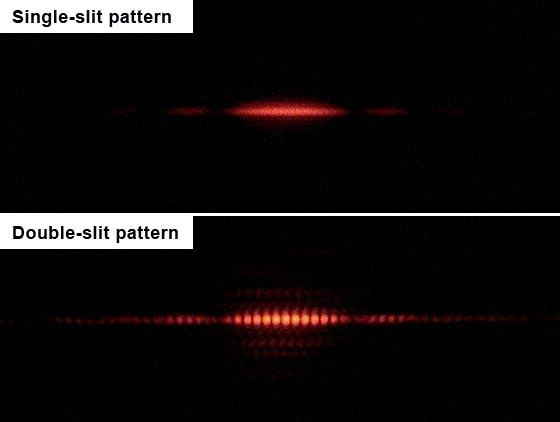
\includegraphics[width=\linewidth, height=1.5in, keepaspectratio]{../figure/double_slit2.jpg}
\caption{In the double slit experiment, opening two slits can actually
cause some positions to receive \emph{fewer} electrons than before.}
\label{tmplabelfig}
\end{marginfigure}

Quantum mechanics is a mathematical theory that allows us to calculate
and predict the results of this and many other examples. If you think of
quantum as an explanation as to what ``really'' goes on in the world, it
can be rather confusing. However, if you simply ``shut up and
calculate'' then it works amazingly well at predicting the results of a
great many experiments.

In the double slit experiment, quantum mechanics still allows to compute
numbers \(\alpha\) and \(\beta\) that denote ``probabilities'' that the
first and second electrons hit the detector. The only difference that in
quantum mechanics these probabilities might be \emph{negative} numbers.
However, probabilities can only be negative when no one is looking at
them. When we actually measure what happened to the detector, we make
the probabilities positive by \emph{squaring} them. So, if only the
first slit is open, the detector will be hit \(\alpha^2\) fraction of
the time. If only the second slit is open, the detector will be hit
\(\beta^2\) fraction of the time. And if both slits are open, the
detector will be hit \((\alpha+\beta)^2\) fraction of the time. Note
that it can well be that \((\alpha+\beta)^2 < \alpha^2 + \beta^2\) and
so this calculation explains why the number of times a detector is hit
when two slits are open might be \emph{smaller} than the number of times
it is hit when either slit is open. If you haven't seen it before, it
may seem like complete nonsense and at this point I'll have to politely
point you back to the part where I said we should not question quantum
mechanics but simply ``shut up and calculate''.\footnote{If you
  \emph{have} seen quantum mechanics before, I should warn that I am
  making here many simplifications. In particular in quantum mechanics
  the ``probabilities'' can actually be \emph{complex} numbers, though
  one gets most of the qualitative understanding by considering them as
  potentially negative real numbers. I will also be focusing throughout
  this presentation on so called ``pure'' quantum states, and ignore the
  fact that generally the states of a quantum subsystem are \emph{mixed}
  states that are a convex combination of pure states and can be
  described by a so called \emph{density matrix}. This issue does not
  arise as much in quantum algorithms precisely because the goal is for
  a quantum computer is to be an isolated system that can evolve to
  continue to be in a pure state; in real world quantum computers
  however there will be interference from the outside world that causes
  the state to become mixed and increase its so called ``von Neumann
  entropy''- fighting this interference and the second law of
  thermodynamics is much of what the challenge of building quantum
  computers is all about . More generally, this lecture is not meant to
  be a complete or accurate description of quantum mechanics, quantum
  information theory, or quantum computing, but rather just give a sense
  of the main points that are different about it from classical
  computing and how they relate to cryptography.}

Some of the counterintuitive properties that arise from these negative
probabilities include:

\begin{itemize}
\tightlist
\item
  \textbf{Interference} - As we see here, probabilities can ``cancel
  each other out''.
\item
  \textbf{Measurement} - The idea that probabilities are negative as
  long as ``no one is looking'' and ``collapse'' to positive
  probabilities when they are \emph{measured} is deeply disturbing.
  Indeed, people have shown that it can yield to various strange
  outcomes such as ``spooky actions at a distance'', where we can
  measure an object at one place and instantaneously (faster than the
  speed of light) cause a difference in the results of a measurements in
  a place far removed. Unfortunately (or fortunately?) these strange
  outcomes have been confirmed experimentally.
\item
  \textbf{Entanglement} - The notion that two parts of the system could
  be connected in this weird way where measuring one will affect the
  other is known as \emph{quantum entanglement}.
\end{itemize}

Again, as counter-intuitive as these concepts are, they have been
experimentally confirmed, so we just have to live with them.

\subsection{Quantum computing and computation - an executive
summary.}\label{Quantum-computing-and-computat}

One of the strange aspects of the quantum-mechanical picture of the
world is that unlike in the billiard ball example, there is no obvious
algorithm to simulate the evolution of \(n\) particles over \(t\) time
periods in \(poly(n,t)\) steps. In fact, the natural way to simulate
\(n\) quantum particles will require a number of steps that is
\emph{exponential} in \(n\). This is a huge headache for scientists that
actually need to do these calculations in practice.

In the 1981, physicist Richard Feynman proposed to ``turn this lemon to
lemonade'' by making the following almost tautological observation:

\begin{quote}
\emph{If a physical system cannot be simulated by a computer in \(T\)
steps, the system can be considered as performing a computation that
would take more than \(T\) steps}
\end{quote}

So, he asked whether one could design a quantum system such that its
outcome \(y\) based on the initial condition \(x\) would be some
function \(y=f(x)\) such that \textbf{(a)} we don't know how to
efficiently compute in any other way, and \textbf{(b)} is actually
useful for something.\footnote{As its title suggests, Feynman's
  \href{https://www.cs.berkeley.edu/~christos/classics/Feynman.pdf}{lecture}
  was actually focused on the other side of simulating physics with a
  computer, but he mentioned that as a ``side remark'' one could wonder
  if it's possible to simulate physics with a new kind of computer - a
  ``quantum computer'' which would ``not {[}be{]} a Turing machine, but
  a machine of a different kind''. As far as I know, Feynman did not
  suggest that such a computer could be useful for computations
  completely outside the domain of quantum simulation, and in fact he
  found the question of whether quantum mechanics could be simulated by
  a classical computer to be more interesting.} In 1985, David Deutsch
formally suggested the notion of a quantum Turing machine, and the model
has been since refined in works of Detusch and Josza and Bernstein and
Vazirani. Such a system is now known as a \emph{quantum computer}.

For a while these hypothetical quantum computers seemed useful for one
of two things. First, to provide a general-purpose mechanism to simulate
a variety of the real quantum systems that people care about. Second, as
a challenge to the theory of computation's approach to model efficient
computation by Turing machines, though a challenge that has little
bearing to practice, given that this theoretical ``extra power'' of
quantum computer seemed to offer little advantage in the problems people
actually want to solve such as combinatorial optimization, machine
learning, data structures, etc..

To a significant extent, this is still true today. We have no real
evidence that quantum computers, if built, will offer truly
significant\footnote{I am using the theorist' definition of conflating
  ``significant'' with ``super-polynomial''. As we'll see, Grover's
  algorithm does offer a very generic \emph{quadratic} advantage in
  computation. Whether that quadratic advantage will ever be good enough
  to offset in practice the significant overhead in building a quantum
  computer remains an open question. We also don't have evidence that
  super-polynomial speedups \emph{can't} be achieved for some problems
  outside the Factoring/Dlog or quantum simulation domains, and there is
  at least \href{http://www.dwavesys.com/}{one company} banking on such
  speedups actually being feasible.} advantage in 99 percent of the
applications of computing.\footnote{This ``99 percent'' is a figure of
  speech, but not completely so. It seems that for many web servers, the
  TLS protocol (which based on the current non-lattice based systems
  would be completely broken by quantum computing) is responsible
  \href{https://goo.gl/Gekjrc}{for about 1 percent of the CPU usage}.}
However, there is one cryptography-sized exception: In 1994 Peter Shor
showed that quantum computers can solve the integer factoring and
discrete logarithm in polynomial time. This result has captured the
imagination of a great many people, and completely energized research
into quantum computing.\\
This is both because the hardness of these particular problems provides
the foundations for securing such a huge part of our communications (and
these days, our economy), as well as it was a powerful demonstration
that quantum computers could turn out to be useful for problems that
a-priori seemd to have nothing to do with quantum physics. As we'll
discuss later, at the moment there are several intensive efforts to
construct large scale quantum computers. It seems safe to say that, as
far as we know, in the next five years or so there will not be a quantum
computer large enough to factor, say, a \(1024\) bit number, but it is
quite possible that some quantum computer will be built that is strong
enough to achieve some task that is too inefficient to achieve with a
non-quantum or ``classical'' computer (or at least requires more
resources classically than it would for this computer). When and if such
a computer is built that can break reasonable parameters of Diffie
Hellman, RSA and elliptic curve cryptography is anybody's guess. It
could also be a ``self destroying prophecy'' whereby the existence of a
small-scale quantum computer would cause everyone to shift away to
lattice-based crypto which in turn will diminish the motivation to
invest the huge resources needed to build a large scale quantum
computer.\footnote{Of course, given that
  \href{http://blog.cryptographyengineering.com/2016/03/attack-of-week-drown.html}{we're
  still hearing} of attacks exploiting ``export grade'' cryptography
  that was supposed to disappear with 1990's, I imagine that we'll still
  have products running 1024 bit RSA when everyone has a quantum laptop.}

The above summary might be all that you need to know as a cryptographer,
and enough motivation to study lattice-based cryptography as we do in
this course. However, because quantum computing is such a beautiful and
(like cryptography) counter-intuitive concept, we will try to give at
least a hint of what it is about and how Shor's algorithm works.

\section{Quantum 101}\label{Quantum-}

We now present some of the basic notions in quantum information. It is
very useful to contrast these notions to the setting of
\emph{probabilistic} systems and see how ``negative probabilities'' make
a difference. This discussion is somewhat brief. The chapter on quantum
computation in my \href{http://theory.cs.princeton.edu/complexity/}{book
with Arora} (see
\href{http://theory.cs.princeton.edu/complexity/ab_quantumchap.pdf}{draft
here}) is one relatively short resource that contains essentially
everything we discuss here. See also this
\href{http://www.scottaaronson.com/blog/?p=208}{blog post of Aaronson}
for a high level explanation of Shor's algorithm which ends with links
to several more detailed expositions. See also
\href{http://www.scottaaronson.com/democritus/lec14.html}{this lecture}
of Aaronson for a great discussion of the feasibility of quantum
computing (Aaronson's
\href{http://www.scottaaronson.com/democritus/default.html}{course
lecture notes} and the
\href{http://www.amazon.com/Quantum-Computing-since-Democritus-Aaronson/dp/0521199565}{book}
that they spawned are fantastic reads as well).

\paragraph{States:} We will consider a simple quantum system that
includes \(n\) objects (e.g., electrons/photons/transistors/etc..) each
of which can be in either an ``on'' or ``off'' state - i.e., each of
them can encode a single \emph{bit} of information, but to emphasize the
``quantumness'' we will call it a \emph{qubit}. A \emph{probability
distribution} over such a system can be described as a \(2^n\)
dimensional vector \(v\) with non-negative entries summing up to \(1\),
where for every \(x\in\{0,1\}^n\), \(v_x\) denotes the probability that
the system is in state \(x\). As we mentioned, quantum mechanics allows
negative (in fact even complex) probabilities and so a \emph{quantum
state} of the system can be described as a \(2^n\) dimensional vector
\(v\) such that \(\|v\|^2 = \sum_x |v_x|^2 = 1\).

\paragraph{Measurement:} Suppose that we were in the classical
probabilistic setting, and that the \(n\) bits are simply random coins.
Thus we can describe the \emph{state} of the system by the
\(2^n\)-dimensional vector \(v\) such that \(v_x=2^{-n}\) for all \(x\).
If we \emph{measure} the system and see what the coins came out, we will
get the value \(x\) with probability \(v_x\). Naturally, if we measure
the system twice we will get the same result. Thus, after we see that
the coin is \(x\), the new state of the system \emph{collapses} to a
vector \(v\) such that \(v_y = 1\) if \(y=x\) and \(v_y=0\) if
\(y\neq x\). In a quantum state, we do the same thing: if we
\emph{measure} a vector \(v\) corresponds to turning it with probability
\(|v_x|^2\) into a vector that has \(1\) on coordinate \(x\) and zero on
all the other coordinates.

\paragraph{Operations:} In the classical probabilistic setting, if we
have a system in state \(v\) and we apply some function
\(f:\{0,1\}^n\rightarrow\{0,1\}^n\) then this transforms \(v\) to the
state \(w\) such that \(w_y = \sum_{x:f(x)=y} v_x\).\\
Another way to state this, is that \(w=M_f\) where \(M_f\) is the matrix
such that \(M_{f(x),x}=1\) for all \(x\) and all other entries are
\(0\). If we toss a coin and decide with probability \(1/2\) to apply
\(f\) and with probability \(1/2\) to apply \(g\), this corresponds to
the matrix \((1/2)M_f + (1/2)M_g\). More generally, the set of
operations that we can apply can be captured as the set of convex
combinations of all such matrices- this is simply the set of
non-negative matrices whose columns all sum up to \(1\)- the
\emph{stochastic} matrices. In the quantum case, the operations we can
apply to a quantum state are encoded as a \emph{unitary} matrix, which
is a matrix \(M\) such that \(\|Mv\|=\|v\|\) for all vectors \(v\).

\paragraph{Elementary operations:} Of course, even in the probabilistic
setting, not every function \(f:\{0,1\}^n\rightarrow\{0,1\}^n\) is
efficiently computable. We think of a function as efficiently computable
if it is composed of polynomially many elementary operations, that
involve at most \(2\) or \(3\) bits or so (i.e., Boolean \emph{gates}).
That is, we say that a matrix \(M\) is \emph{elementary} if it only
modifies three bits. That is, \(M\) is obtained by ``lifting'' some
\(8\times 8\) matrix \(M'\) that operates on three bits \(i,j,k\),
leaving all the rest of the bits intact. Formally, given an
\(8\times 8\) matrix \(M'\) (indexed by strings in \(\{0,1\}^3\)) and
three distinct indices \(i<j<k \in \{1,\ldots,n\}\) we define the
\emph{\(n\)-lift of \(M'\) with indices \(i,j,k\)} to be the
\(2^n\times 2^n\) matrix \(M\) such that for every strings \(x\) and
\(y\) that agree with each other on all coordinates except possibly
\(i,j,k\), \(M_{x,y}=M'_{x_ix_jx_k,y_iy_jy_k}\) and otherwise
\(M_{x,y}=0\). Note that if \(M'\) is of the form \(M'_f\) for some
function \(f:\{0,1\}^3\rightarrow\{0,1\}^3\) then \(M=M_g\) where
\(g:\{0,1\}^n\rightarrow\{0,1\}^n\) is defined as \(g(x)=f(x_ix_jx_k)\).
We define \(M\) as an \emph{elementary stochastic matrix} or a
\emph{probabilistic gate} if \(M\) is equal to an \(n\) lift of some
stochastic \(8\times 8\) matrix \(M'\). The quantum case is similar: a
\emph{quantum gate} is a \(2^n\times 2^n\) matrix that is an \(N\) lift
of some unitary \(8\times 8\) matrix \(M'\). It is an exercise to prove
that lifting preserves stochasticity and unitarity. That is, every
probabilistic gate is a stochastic matrix and every quantum gate is a
unitary matrix.

\paragraph{Complexity:} For every stochastic matrix \(M\) we can define
its \emph{randomized complexity}, denoted as \(R(M)\) to be the minimum
number \(T\) such that \(M\) is can be (approximately) obtained by
combining \(T\) elementary probabilistic gates. To be concrete, we can
define \(R(M)\) to be the minimum \(T\) such that there exists \(T\)
elementary matrices \(M_1,\ldots,M_T\) such that for every \(x\),
\(\sum_y |M_{y,x}-(M_T\cdots M_1)_{y,x}|<0.1\). (It can be shown that
\(R(M)\) is finite and in fact at most \(10^n\) for every \(M\); we can
do so by writing \(M\) as a convex combination of function and writing
every function as a composition of functions that map a single string
\(x\) to \(y\), keeping all other inputs intact.) We will say that a
probabilistic process \(M\) mapping distributions on \(\{0,1\}^n\) to
distributions on \(\{0,1\}^n\) is \emph{efficiently classically
computable} if \(R(M) \leq poly(n)\). If \(M\) is a unitary matrix, then
we define the \emph{quantum complexity} of \(M\), denoted as \(Q(M)\),
to be the minimum number \(T\) such that there are quantum gates
\(M_1,\ldots,M_T\) satisfying that for every \(x\),
\(\sum_y |M_{y,x}-(M_T \cdots M_1)_{y,x}|^2 < 0.1\).\\
We say that \(M\) is \emph{efficiently quantumly computable} if
\(Q(M)\leq poly(n)\).

\paragraph{Computing functions:} We have defined what it means for an
operator to be probabilistically or quantumly efficiently computable,
but we typically are interested in computing some function
\(f:\{0,1\}^m\rightarrow\{0,1\}^\ell\). The idea is that we say that
\(f\) is efficiently computable if the corresponding operator is
efficiently computable, except that we also allow to use extra memory
and so to embed \(f\) in some \(n=poly(m)\). We define \(f\) to be
\emph{efficiently classically computable} if there is some \(n=poly(m)\)
such that the operator \(M_g\) is efficiently classically computable
where \(g:\{0,1\}^n\rightarrow\{0,1\}^n\) is defined such that
\(g(x_1,\ldots,x_n)=f(x_1,\ldots,x_m)\). In the quantum case we have a
slight twist since the operator \(M_g\) is not necessarily a unitary
matrix.\footnote{It is a good exercise to verify that for every
  \(g:\{0,1\}^n\rightarrow\{0,1\}^n\), \(M_g\) is unitary if and only if
  \(g\) is a permutation.} Therefore we say that \(f\) is
\emph{efficiently quantumly computable} if there is \(n=poly(m)\) such
that the operator \(M_q\) is efficiently quantumly computable where
\(g:\{0,1\}^n\rightarrow\{0,1\}^n\) is defined as
\(g(x_1,\ldots,x_n) = x_1\cdots x_m \|( f(x_1\cdots x_m)0^{n-m-\ell}\; \oplus \; x_{m+1}\cdots x_n)\).

\paragraph{Quantum and classical computation:} The way we defined what
it means for a function to be efficiently quantumly computable, it might
not be clear that if \(f:\{0,1\}^m\rightarrow\{0,1\}^\ell\) is a
function that we can compute by a polynomial size Boolean circuit (e.g.,
combining polynomially many AND, OR and NOT gates) then it is also
quantumly efficiently computable. The idea is that for every gate
\(g:\{0,1\}^2\rightarrow\{0,1\}\) we can define an \(8\times 8\) unitary
matrix \(M_h\) where \(h:\{0,1\}^3\rightarrow\{0,1\}^3\) has the form
\(h(a,b,c)=a,b,c\oplus g(a,b)\). So, if \(f\) has a circuit of \(s\)
gates, then we can dedicate an extra bit for every one of these gates
and then run the corresponding \(s\) unitary operations one by one, at
the end of which we will get an operator that computes the mapping
\(x_1,\ldots,x_{m+\ell+s} = x_1\cdots x_m \| x_{m+1}\cdots x_{m+s} \oplus f(x_1,\ldots,x_m)\|g(x_1\ldots x_m)\)
where the the \(\ell+i^{th}\) bit of \(g(x_1,\ldots,x_n)\) is the result
of applying the \(i^{th}\) gate in the calculation of
\(f(x_1,\ldots,x_m)\). So this is ``almost'' what we wanted except that
we have this ``extra junk'' that we need to get rid of. The idea is that
we now simply run the same computation again which will basically we
mean we XOR another copy of \(g(x_1,\ldots,x_m)\) to the last \(s\)
bits, but since \(g(x)\oplus g(x) = 0^s\) we get that we compute the map
\(x \mapsto x_1\cdots x_m \| (f(x_1,\ldots,x_m)0^s \;\oplus\; x_{m+1}\cdots x_{m+\ell+s})\)
as desired.

\paragraph{The "obviously exponential" fallacy:} A priori it might seem
``obvious'' that quantum computing is exponentially powerful, since to
compute a quantum computation on \(n\) bits we need to maintain the
\(2^n\) dimensional state vector and apply \(2^n\times 2^n\) matrices to
it. Indeed popular descriptions of quantum computing (too) often say
something along the lines that the difference between quantum and
classical computer is that a classic bit can either be zero or one while
a qubit can be in both states at once, and so in many qubits a quantum
computer can perform exponentially many computations at once. Depending
on how you interpret this, this description is either false or would
apply equally well to \emph{probabilistic computation}. However, for
probabilistic computation it is a not too hard exercise to show that if
\(f:\{0,1\}^m\rightarrow\{0,1\}^n\) is an efficiently computable
function then it has a polynomial size circuit of AND, OR and NOT
gates.\footnote{It is a good exercise to show that if \(M\) is a
  probabilistic process with \(R(M) \leq T\) then there exists a
  probabilistic circuit of size, say, \(100 T n^2\) that approximately
  computes \(M\) in the sense that for every input \(x\),
  \(\sum_{y\in\{0,1\}^n} \left| \Pr[C(x)=y] - M_{x,y} \right| < 1/3\).}
Moreover, this ``obvious'' approach for simulating a quantum computation
will take not just exponential time but \emph{exponential space} as
well, while it is not hard to show that using a simple recursive formula
one can calculate the final quantum state using \emph{polynomial space}
(in physics parlance this is known as ``Feynman path integrals''). So,
the exponentially long vector description by itself does not imply that
quantum computers are exponentially powerful. Indeed, we cannot
\emph{prove} that they are (since in particular we can't prove that
\emph{every} polynomial space calculation can be done in polynomial
time, in complexity parlance we don't know how to rule out that
\(P=\ensuremath{\mathit{PSPACE}}\)), but we do have some problems
(integer factoring most prominently) for which they do provide
exponential speedup over the currently best \emph{known} classical
(deterministic or probabilistic) algorithms.

\subsection{Physically realizing quantum
computation}\label{Physically-realizing-quantum-c}

To realize quantum computation one needs to create a system with \(n\)
independent binary states (i.e., ``qubits''), and be able to manipulate
small subsets of two or three of these qubits to change their state.
While by the way we defined operations above it might seem that one
needs to be able to perform arbitrary unitary operations on these two or
three qubits, it turns out that there several choices for
\emph{universal sets} - a small constant number of gates that generate
all others. The biggest challenge is how to keep the system from being
measured and \emph{collapsing} to a single classical combination of
states. This is sometimes known as the \emph{coherence time} of the
system. The
\href{https://courses.cs.washington.edu/courses/cse599d/06wi/lecturenotes19.pdf}{threshold
theorem} says that there is some absolute constant level of errors
\(\tau\) so that if errors are created at every gate at rate smaller
than \(\tau\) then we can recover from those and perform arbitrary long
computations. (Of course there are different ways to model the errors
and so there are actually several threshold \emph{theorems}
corresponding to various noise models).

There have been several proposals to build quantum computers:

\begin{itemize}
\item
  \href{https://en.wikipedia.org/wiki/Superconducting_quantum_computing}{Superconducting
  quantum computers} use super-conducting electric circuits to do
  quantum computation. \href{http://arxiv.org/abs/1411.7403}{Recent
  works} have shown one can keep these superconducting qubits fairly
  robust to the point one can do some error correction on them (see also
  \href{http://arxiv.org/abs/1508.05882v2}{here}).
\item
  \href{https://en.wikipedia.org/wiki/Trapped_ion_quantum_computer}{Trapped
  ion quantum computers} Use the states of an ion to simulate a qubit.
  People have made some
  \href{http://iontrap.umd.edu/wp-content/uploads/2016/02/1602.02840v1.pdf}{recent
  advances} on these computers too. While it's not clear that's the
  right measuring yard, the
  \href{http://arxiv.org/abs/1507.08852}{current best implementation} of
  Shor's algorithm (for factoring 15) is done using an ion-trap
  computer.
\item
  \href{https://en.wikipedia.org/wiki/Topological_quantum_computer}{Topological
  quantum computers} use a different technology, which is more stable by
  design but arguably harder to manipulate to create quantum computers.
\end{itemize}

These approaches are not mutually exclusive and it could be that
ultimately quantum computers are built by combining all of them
together. I am not at all an expert on this matter, but it seems that
progress has been slow but steady and it is quite possible that we'll
see a 20-50 qubit computer sometime in the next 5-10 years.

\subsection{Bra-ket notation}\label{Bra-ket-notation}

Quantum computing is very confusing and counterintuitive for many
reasons. But there is also a ``cultural'' reason why people sometimes
find quantum arguments hard to follow. Quantum folks follow their own
special
\href{https://en.wikipedia.org/wiki/Bra\%E2\%80\%93ket_notation}{notation}
for vectors. Many non quantum people find it ugly and confusing, while
quantum folks secretly wish they people used it all the time, not just
for non-quantum linear algebra, but also for restaurant bills and
elemntary school math classes.

The notation is actually not so confusing. If \(x\in\{0,1\}^n\) then
\(|x\rangle\) denotes the \(x^{th}\) standard basis vector in \(2^n\)
dimension. That is \(|x\rangle\) \(2^n\)-dimensional column vector that
has \(1\) in the \(x^{th}\) coordinate and zero everywhere else. So, we
can describe the column vector that has \(\alpha_x\) in the \(x^{th}\)
entry as \(\sum_{x\in\{0,1\}^n} \alpha_x |x\rangle\). One more piece of
notation that is useful is that if \(x\in\{0,1\}^n\) and
\(y\in\{0,1\}^m\) then we identify \(|x\rangle|y\rangle\) with
\(|xy\rangle\) (that is, the \(2^{n+m}\) dimensional vector that has
\(1\) in the coordinate corresponding to the concatenation of \(x\) and
\(y\), and zero everywhere else). This is more or less all you need to
know about this notation to follow this lecture.\footnote{If you are
  curious, there is an analog notation for \emph{row} vectors as
  \(\langle x|\). Generally if \(u\) is a vector then \(|u\rangle\)
  would be its form as a column vector and \(\langle u|\) would be its
  form as a row product. Hence since \(u^\top v = \langle u,v \rangle\)
  the inner product of \(u\) and \(b\) can be thought of as
  \(\langle u||v\rangle\) . The \emph{outer product} (the matrix whose
  \(i,j\) entry is \(u_iv_j\)) is denoted as \(|u\rangle\langle v|\).}

A quantum gate is an operation on at most three bits, and so it can be
completely specified by what it does to the \(8\) vectors
\(|000\rangle,\ldots,|111\rangle\). Quantum states are always unit
vectors and so we sometimes omit the normalization for convenience; for
example we will identify the state \(|0\rangle+|1\rangle\) with its
normalized version
\(\tfrac{1}{\sqrt{2}}|0\rangle + \tfrac{1}{\sqrt{2}}|1\rangle\).

\subsection{Bell's Inequality}\label{Bells-Inequality}

There is something weird about quantum mechanics. In 1935
\href{http://plato.stanford.edu/entries/qt-epr/}{Einstein, Podolsky and
Rosen (EPR)} tried to pinpoint this issue by highlighting a previously
unrealized corollary of this theory. It was already realized that the
fact that quantum measurement collapses the state to a definite aspect
yields the \emph{uncertainty principle}, whereby if you measure a
quantum system in one orthogonal basis, you will not know how it would
have measured in an incohrent basis to it (such as position
vs.~momentum). What EPR showed was that quantum mechanics results in so
called ``spooky action at a distance'' where if you have a system of two
particles then measuring one of them would instantenously effect the
state of the other. Since this ``state'' is just a mathematical
description, as far as I know the EPR paper was considered to be a
thought experiment showing troubling aspects of quantum mechanics,
without bearing on experiment. This changed when in 1965 John Bell
showed an actual experiment to test the predictions of EPR and hence pit
intuitive common sense against the predictions of quantum mechanics.
Quantum mechanics won. Nonetheless, since the results of these
experiments are so obviously wrong to anyone that has ever sat in an
armchair, that there are still a number of
\href{http://www.scottaaronson.com/blog/?p=2464}{Bell denialists}
arguing that quantum mechanics is wrong in some way.

So, what is this Bell's Inequality? Suppose that Alice and Bob try to
convince you they have telepathic ability, and they aim to prove it via
the following experiment. Alice and Bob will be in separate closed
rooms.\footnote{If you are extremely paranoid about Alice and Bob
  communicating with one another, you can coordinate with your assistant
  to perform the experiment exactly at the same time, and make sure that
  the rooms are so that Alice and Bob couldn't communicate to each other
  in time the results of the coin even if they do so at the speed of
  light.} You will interrogate Alice and your associate will interrogate
Bob. You choose a random bit \(x\in\{0,1\}\) and your associate chooses
a random \(y\in\{0,1\}\). We let \(a\) be Alice's response and \(b\) be
Bob's response. We say that Alice and Bob win this experiment if
\(a \oplus b = x \wedge y\).

Now if Alice and Bob are not telepathic, then they need to agree in
advance on some strategy. The most general form of such a strategy is
that Alice and Bob agree on some distribution over a pair of functions
\(d,g:\{0,1\}\rightarrow\{0,1\}\), such that Alice will set \(a=f(x)\)
and Bob will set \(b=g(x)\). Therefore, the following claim, which is
basically Bell's Inequality,\footnote{This form of Bell's game was shown
  by CHSH} implies that Alice and Bob cannot succeed in this game with
probability higher than \(3/4\):

\paragraph{Claim:} For every two functions
\(f,g:\{0,1\}\rightarrow\{0,1\}\) there exist some \(x,y\in\{0,1\}\)
such that \(f(x) \oplus g(y) \neq x \wedge y\).

\paragraph{Proof:} Suppose toward a contradiction that \(f,g\) satisfy
\(f(x) \oplus g(y) = x \wedge y \;(*)\) or
\(f(x) = (x \wedge y) \oplus g(y)\;(*)\) ;. So if \(y=0\) it must be
that \(f(x)=0\) for all \(x\), but on the other hand, if \(y=1\) then
for \((*)\) to hold then it must be that \(f(x) = x \oplus g(1)\) but
that means that \(f\) cannot be constant. QED

An amazing \href{http://arxiv.org/abs/1508.05949}{experimentally
verified} fact is that quantum mechanics allows for telepathy:\footnote{More
  accurately, one either has to give up on a ``billiard ball type''
  theory of the universe or believe in telepathy (believe it or not,
  some scientists went for the
  \href{https://en.wikipedia.org/wiki/Superdeterminism}{latter option}).}

\paragraph{Claim:} There is a strategy for Alice and Bob to succeed in
this game with probability at least \(0.8\).

\paragraph{Proof:} The main idea is for Alice and Bob to first prepare a
2-qubit quantum system in the state (up to normalization)
\(|00\rangle+|11\rangle\) (this is known as an \emph{EPR pair}). Alice
takes the first qubit in this system to her room, and Bob takes the
qubit to his room. Now, when Alice receives \(x\) if \(x=0\) she does
nothing and if \(x=1\) she applies the unitary map \(R_{\pi/8}\) to her
qubit where
\(R_\theta = \left( \begin{smallmatrix} cos \theta & \sin -\theta \\ \sin \theta & \cos \theta \end{smallmatrix} \right)\).
When Bob receives \(y\), if \(y=0\) he does nothing and if \(y=1\) he
applies the unitary map \(R_{-\pi/8}\) to his qubit. Then each one of
them measures their qubit and sends this as their response. Recall that
to win the game Bob and Alice want their outputs to be more likely to
differ if \(x=y=1\) and to be more likely to agree otherwise.

If \(x=y=0\) then the state does not change and Alice and Bob always
output either both \(0\) or both \(1\), and hence in both case
\(a\oplus b = x \wedge y\). If \(x=0\) and \(y=1\) then after Alice
measures her bit, if she gets \(0\) then Bob's state is equal to
\(-\cos (\pi/8)|0\rangle-\sin(\pi/8)|1\rangle\) which will equal \(0\)
with probability \(\cos^2 (\pi/8)\). The case that Alice gets \(1\), or
that \(x=1\) and \(y=0\), is symmetric, and so in all the cases where
\(x\neq y\) (and hence \(x \wedge y=0\)) the probability that \(a=b\)
will be \(\cos^2(\pi/8) \geq 0.85\). For the case that \(x=1\) and
\(y=1\), direct calculation via trigonomertic identities yields that all
four options for \((a,b)\) are equally likely and hence in this case
\(a=b\) with probability \(0.5\). The overall probability of winning the
game is at least
\(\tfrac{1}{4}\cdot 1 + \tfrac{1}{2}\cdot 0.85 + \tfrac{1}{4} \cdot 0.5 =0.8\).
QED

\begin{quote}
\textbf{Quantum vs probabilistic strategies:} It is instructive to
understand what is it about quantum mechanics that enabled this gain in
Bell's Inequality. For this, consider the following analogous
probabilistic strategy for Alice and Bob. They agree that each one of
them output \(0\) if he or she get \(0\) as input and outputs \(1\) with
probability \(p\) if they get \(1\) as input. In this case one can see
that their success probability would be
\(\tfrac{1}{4}\cdot 1 + \tfrac{1}{2}(1-p)+\tfrac{1}{4}[2p(1-p)]=0.75 -0.5p^2 \leq 0.75\).
The quantum strategy we described above can be thought of as a variant
of the probabilistic strategy for \(p\) is \(\sin^2 (\pi/8)=0.15\). But
in the case \(x=y=1\), instead of disagreeing only with probability
\(2p(1-p)=1/4\), because we can use these negative probabilities in the
quantum world and rotate the state in opposite directions, the
probability of disagreement ends up being \(\sin^2 (\pi/4)=0.5\).
\end{quote}

\section{Grover's Algorithm}\label{Grovers-Algorithm}

Shor's Algorithm, which we'll see in the next lecture, is an amazing
achievement, but it only applies to very particular problems. It does
not seem to be relevant to breaking AES, lattice based cryptography, or
problems not related to quantum computing at all such as scheduling,
constraint satisfaction, traveling salesperson etc.. etc.. Indeed, for
the most general form of these search problems, classically we don't how
to do anything much better than brute force search, which takes \(2^n\)
time over an \(n\)-bit domain. Lev Grover showed that quantum computers
can obtain a quadratic improvement over this brute force search, solving
SAT in \(2^{n/2}\) time. The effect of Grover's algorithm on
cryptography is fairly mild: one essentially needs to double the key
lengths of symmetric primitives. But beyond cryptography, if large scale
quantum computers end up being built, Grover search and its variants
might end up being some of the most useful computational problems they
will tackle. Grover's theorem is the following:

\paragraph{Theorem (Grover search , 1996):} There is a quantum
\(O(2^{n/2}poly(n))\)-time algorithm that given a \(poly(n)\)-sized
circuit computing a function \(f:\{0,1\}^n\rightarrow\{0,1\}\) outputs a
string \(x^*\in\{0,1\}^n\) such that \(f(x^*)=1\).

\paragraph{Proof sketch:} The proof is not hard but we only sketch it
here. The general idea can be illustrated in the case that there exists
a single \(x^*\) satisfying \(f(x^*)=1\). (There is a classical
reduction from the general case to this problem.) As in Simon's
algorithm, we can efficiently initialize an \(n\)-qubit system to the
uniform state \(u = 2^{-n/2}\sum_{x\in\{0,1\}^n}|x\rangle\) which has
\(2^{-n/2}\) dot product with \(|x^*\rangle\). Of course if we measure
\(u\), we only have probability \((2^{-n/2})^2 = 2^{-n}\) of obtaining
the value \(x^*\). Our goal would be to use \(O(2^{n/2})\) calls to the
oracle to transform the system to a state \(v\) with dot product at
least some constant \(\epsilon>0\) with the state \(|x^*\rangle\).

It is an exercise to show that using \(Had\) gets we can efficiently
compute the unitary operator \(U\) such that \(Uu = u\) and \(Uv = -v\)
for every \(v\) orthogonal to \(u\). Also, using the circuit for \(f\),
we can efficiently compute the unitary operator \(U^*\) such that
\(U^*|x\rangle=|x\rangle\) for all \(x\neq x^*\) and
\(U^*|x^*\rangle=-|x^*\rangle\). It turns out that \(O(2^{n/2})\)
applications of \(\ensuremath{\mathit{UU}}^*\) to \(u\) yield a vector
\(v\) with \(\Omega(1)\) inner product with \(|x^*\rangle\). To see why,
consider what these operators do in the two dimensional linear subspace
spanned by \(u\) and \(|x^*\rangle\). (Note that the initial state \(u\)
is in this subspace and all our operators preserve this property.) Let
\(u_\perp\) be the unit vector orthogonal to \(u\) in this subspace and
let \(x^*_\perp\) be the unit vector orthogonal to \(|x^*\rangle\) in
this subspace. Restricted to this subspace, \(U^*\) is a reflection
along the axis \(x^*_\perp\) and \(U\) is a reflection along the axis
\(u\).

Now, let \(\theta\) be the angle between \(u\) and \(x^*_\perp\). These
vectors are very close to each other and so \(\theta\) is very small but
not zero - it is equal to \(\sin^{-1}( 2^{-n/2})\) which is roughly
\(2^{-n/2}\). Now if our state \(v\) has angle \(\alpha \geq 0\) with
\(u\), then as long as \(\alpha\) is not too large (say
\(\alpha<\pi/8\)) then this means that \(v\) has angle \(u+\theta\) with
\(x^*_\perp\). That means that \(U^*v\) will have angle
\(-\alpha-\theta\) with \(x^*_\perp\) or \(-\alpha-2\theta\) with \(u\),
and hence \(\ensuremath{\mathit{UU}}^*v\) will have angle
\(\alpha+2\theta\) with \(u\). Hence in one application from
\(\ensuremath{\mathit{UU}}^*\) we move \(2\theta\) radians away from
\(u\), and in \(O(2^{-n/2})\) steps the angle between \(u\) and our
state will be at least some constant \(\epsilon>0\). Since we live in
the two dimensional space spanned by \(u\) and \(|x\rangle\), it would
mean that the dot product of our state and \(|x\rangle\) will be at
least some constant as well. QED
